\chapter{Mogelijke oplossingen}
\label{Mogelijke_oplossingen}
%%%%%%%%%%%%%%%%%%%%%%%%%%%%%%%%%%%%%%%%%%%%%%%%%%%%%%%%%%%%%%%%%%%%%%%%

%%%%%%%%%%%%%%%%%%%%%%%%%%%%%%%%%%%%%%%%%%%%%%%%%%%%%%%%%%%%%%%%%%%%%%%%
\section{Extruder problemen}
%%%%%%%%%%%%%%%%%%%%%%%%%%%%%%%%%%%%%%%%%%%%%%%%%%%%%%%%%%%%%%%%%%%%%%%%

Het probleem van een vastlopende extruder kwam voor met een direct drive
extruder. Een oplossing die overwogen was, was het overstappen naar een andere
extruder architectuur.

%%%%%%%%%%%%%%%%%%%%%%%%%%%%%%%%%%%%%%%%%%%%%%%%%%%%%%%%%%%%%%%%%%%%%%%%
\subsection{Verschillende soorten extruders}
%%%%%%%%%%%%%%%%%%%%%%%%%%%%%%%%%%%%%%%%%%%%%%%%%%%%%%%%%%%%%%%%%%%%%%%%

\begin{figure}[h]
    \centerline{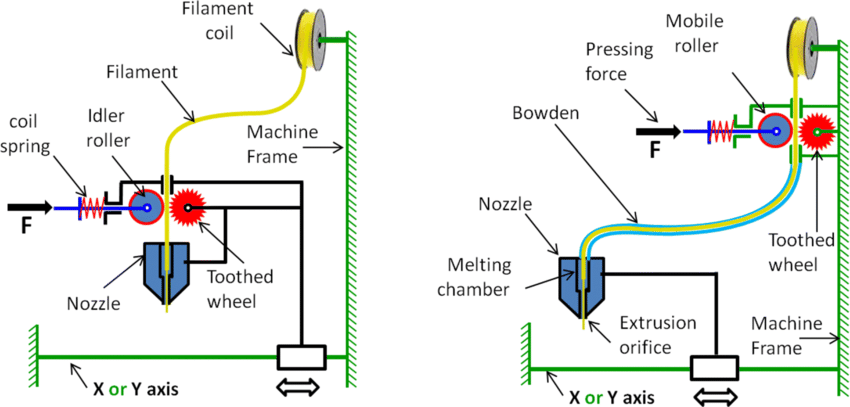
\includegraphics[width=0.85\textwidth]{Basic-diagram-of-FDM-3D-printer-extruder-a-Direct-extruder-b-Bowden-extruder}}
    \caption{Diagram van de twee soorten extruders die veel woorden gebruikt \cite{soorten_extruders}.}
    \label{fig:soorten_extruders}
\end{figure}

%%%%%%%%%%%%%%%%%%%%%%%%%%%%%%%%%%%%%%%%%%%%%%%%%%%%%%%%%%%%%%%%%%%%%%%%
\subsubsection{Bowden extruder}
\label{ss:Bowden_extruder}
%%%%%%%%%%%%%%%%%%%%%%%%%%%%%%%%%%%%%%%%%%%%%%%%%%%%%%%%%%%%%%%%%%%%%%%%

De rechter helft van Figuur \ref{fig:soorten_extruders} \cite{soorten_extruders}
is een diagram van een Bowden extruder. Hierbij is te zien dat \ac{extruder} los
is van de \ac{hotend}.

% uitleg

%%%%%%%%%%%%%%%%%%%%%%%%%%%%%%%%%%%%%%%%%%%%%%%%%%%%%%%%%%%%%%%%%%%%%%%%
\subsubsection{Direct drive extruder}
\label{ss:direct_drive_extruder}
%%%%%%%%%%%%%%%%%%%%%%%%%%%%%%%%%%%%%%%%%%%%%%%%%%%%%%%%%%%%%%%%%%%%%%%%

De linker helft van Figuur \ref{fig:soorten_extruders} \cite{soorten_extruders}
is een diagram van een direct drive extruder.

% uitleg

%%%%%%%%%%%%%%%%%%%%%%%%%%%%%%%%%%%%%%%%%%%%%%%%%%%%%%%%%%%%%%%%%%%%%%%%
\subsection{Zou een Bowden extruder de problemen oplossen}
%%%%%%%%%%%%%%%%%%%%%%%%%%%%%%%%%%%%%%%%%%%%%%%%%%%%%%%%%%%%%%%%%%%%%%%%

Met een bowden extruder zou het probleem van smeltend plastic in de extruder
(Hoofdstuk \ref{s:smeltendplastic}) opgelost kunnen woorden. Echter was
opgemerkt dat PP niet geprint kan woorden met een bowden printer (Hoofdstuk
\ref{s:Dubbelvouwend}).

%%%%%%%%%%%%%%%%%%%%%%%%%%%%%%%%%%%%%%%%%%%%%%%%%%%%%%%%%%%%%%%%%%%%%%%%
\subsection{Zou een water gekoelde extruder de problemen oplossen}
%%%%%%%%%%%%%%%%%%%%%%%%%%%%%%%%%%%%%%%%%%%%%%%%%%%%%%%%%%%%%%%%%%%%%%%%

Een water gekoelde extruder/hotend zou allebei de problemen kunnen oplossen met
als enige nadeel extra complexheid in de vorm van aanstuur elektronica en
software voor de waterkoeling en de waterkoeling zelf (buizen, pomp, radiator).

Een goede optie zou de "Titan Aqua" \cite{titanaqua} zijn.

% bronvermedling naar pagina over watergekoelde hotend/extruder

%%%%%%%%%%%%%%%%%%%%%%%%%%%%%%%%%%%%%%%%%%%%%%%%%%%%%%%%%%%%%%%%%%%%%%%%
\section{Temperatuur overshoot}
%%%%%%%%%%%%%%%%%%%%%%%%%%%%%%%%%%%%%%%%%%%%%%%%%%%%%%%%%%%%%%%%%%%%%%%%

Een \ac{PID} lus voor de kamertemperatuur kan woorden geïmplementeerd in de
firmware van de printer, het vermogen van de warmte-elementen kan worden
teruggedraaid om ervoor te zorgen dat de temperatuur minder snel stijgt en er
dus een minder groot verschil is tussen de gemeenten en de werkelijke
temperatuur.
